\documentclass[11pt]{article}

\usepackage[margin=1in]{geometry}
\usepackage{setspace}
\usepackage{graphicx}
\usepackage{booktabs}
\usepackage{amsmath}
\usepackage{hyperref}
\usepackage{enumitem}
\usepackage{natbib}
\usepackage{fancyvrb}
\usepackage{float}
\usepackage{tikz}
\usetikzlibrary{arrows.meta,positioning,shapes.geometric,calc}

\usepackage{tcolorbox}
\tcbset{
  colback=gray!8,
  colframe=gray!50,
  boxrule=0.4pt,
  arc=2pt,
  left=4pt,
  right=4pt,
  top=4pt,
  bottom=4pt
}

\usepackage{etoolbox}
\AtBeginEnvironment{Verbatim}{\singlespacing}

\renewcommand{\thesection}{}
\setcounter{secnumdepth}{0}

\onehalfspacing
\hypersetup{
  colorlinks=true,
  linkcolor=blue,
  citecolor=blue,
  urlcolor=blue
}

\newcommand{\CompanionRepo}{https://github.com/crossley/crossleylab/tree/main/code/behavioural_experiment_progression}


\title{Behavioural Experiments as State-Driven Execution Systems}

\author{Matthew J. Crossley\\
\small School of Psychological Sciences, Macquarie University, Sydney, Australia \\
\small Performance and Expertise Research Centre, Macquarie University, Sydney, Australia \\
\small Macquarie Minds and Intelligences Initiative, Macquarie University, Sydney, Australia \\
\small \texttt{matthew.crossley@mq.edu.au}}

\date{}

\begin{document}
\maketitle

\begin{abstract}
    ...
\end{abstract}

\section{Introduction}
Behavioural experiments are typically described as ordered
sequences of events in which stimuli are presented,
responses are collected, and trials advance from one stage
to the next. This sequential description is natural for
communicating experimental design and specifying task
procedures, and it provides an effective representation for
many experimental paradigms. However, as experiments become
interactive, adaptive, or contingent on participant
behaviour, sequential descriptions alone can become less
suited to expressing how experimental behaviour is organised
during execution.

Behavioural experiments can instead be viewed as control
problems in which experimental behaviour evolves over time
in response to internal conditions, elapsed time, and
participant input. At any moment during an experiment, the
system occupies a particular mode of operation: stimuli may
be visible or absent, responses may be accepted or ignored,
and timing constraints determine when changes in behaviour
are permitted. Experimental design therefore involves
specifying not only the order of events, but also the
conditions under which behaviour changes from one phase of a
task to another.

From this perspective, behavioural experiments can be
usefully understood as finite state machines
(\citealp{harel_statecharts_1987}) in which experimental
behaviour emerges from transitions between task states
governed by timing and events. In this abstraction, a state
corresponds to a phase of the experiment during which
behavioural rules remain stable. For example, fixation
display, stimulus presentation, response collection, and
feedback can each be understood as distinct states defined
by the stimuli presented, responses monitored, and timing
constraints applied. Transitions between states occur when
specified conditions are satisfied, such as the passage of
time, the detection of a response, or the outcome of a
task-dependent rule. This state-based view does not replace
sequential descriptions of tasks, but provides a more
general representation for reasoning about experimental
control when tasks involve branching logic, adaptive
structure, or ongoing interaction.

State-based representations of behaviour are widely used in
computer science and engineering to describe interactive and
event-driven systems, including user interfaces, robotics,
and game systems (e.g., \citealp{harel_statecharts_1987,
gamma_design_1994}).  The present work does not introduce a
new computational model. Instead, it adopts this established
abstraction as a way of representing experimental control,
making explicit a level of structure that is often implicit
in behavioural experiment design.

Representing experiments in this way allows sequential task
structures to be understood as a special case in which
transitions occur in a fixed order, while more complex
paradigms introduce conditional or event-driven transitions
between states. Describing experimental structure at this
level focuses attention on relationships between task
phases and the conditions governing movement between them,
rather than on particular programming constructs.

Importantly, this state-based description functions as an
abstraction for reasoning about experimental design rather
than as a prescription for implementation. Many existing
experiment frameworks and programming environments already
embody similar control structures internally, although these
structures are often implicit within software abstractions
(e.g., \citealp{brainard_psychophysics_1997,
peirce_psychopypsychophysics_2007, peirce_psychopy2_2019,
mathot_opensesame_2012, krause_expyriment_2014}).  Making
the state structure explicit provides a way to align
conceptual task design with implementation while remaining
independent of specific tools or programming languages.

\section{From Sequential Tasks to State-Structured Control}

Behavioural experiments are commonly specified as ordered
sequences of events. A typical description might state that
a fixation stimulus is presented, followed by a target,
after which a response is collected and feedback is shown
before the next trial begins. This sequential description is
both natural and useful, as it mirrors the intended
structure of the task from the perspective of the
experimenter and participant.

\begin{tcolorbox}[title=Sequential Task Pseudocode]
\begin{Verbatim}[fontsize=\small]
For each trial:

    show_fixation()
    wait(fixation_duration)

    show_stimulus()
    response = wait_for_response(timeout)

    show_feedback(response)
    wait(feedback_duration)
\end{Verbatim}
\end{tcolorbox}

This formulation remains clear when each phase of the task
has a single outcome. As additional contingencies are
introduced, however, the conditions governing progression
between phases become distributed across multiple parts of
the sequence. Behavioural rules that determine when a phase
ends or how the task proceeds must be incorporated into
different functions and locations within the program,
making the overall structure of task flow progressively less
explicit.

To illustrate this, consider a simple reaction time task in
which a fixation stimulus is followed by a target, after
which a response is collected and feedback is presented. In
its simplest form, the task can be implemented directly using
a sequential structure:

\begin{tcolorbox}[title=Sequential Reaction Time Task Pseudocode]
\begin{Verbatim}[fontsize=\small]
For each trial:

    show_fixation()
    wait(fixation_duration)

    show_stimulus()
    response = wait_for_response(timeout)

    show_feedback(response)
    wait(feedback_duration)
\end{Verbatim}
\end{tcolorbox}

Many experiments can be implemented effectively in this way.
As additional task requirements are introduced, however,
behavioural rules must be incorporated into different parts
of the sequence. For example, suppose responses made before
stimulus onset should be treated as anticipations and
terminate the trial early. A natural extension is to
introduce an additional check during the fixation period:

\begin{tcolorbox}[title=Sequential Reaction Time Task with Anticipation Pseudocode]
\begin{Verbatim}[fontsize=\small]
show_fixation()

if keypress occurs during fixation:
    show_feedback("Too early")
    continue to next trial
\end{Verbatim}
\end{tcolorbox}

The logic remains straightforward, but the conditions
governing trial progression are now distributed across more
than one part of the code. Further extensions introduce
additional branching. During stimulus presentation, the
experiment must distinguish between correct responses,
incorrect responses, and failures to respond before a
deadline:

\begin{tcolorbox}[title=Sequential Reaction Time Task with Response Evaluation Pseudocode]
\begin{Verbatim}[fontsize=\small]
show_stimulus()
response = wait_for_response(timeout)

if response == NO_RESPONSE:
    show_feedback("Too slow")

else if response is correct:
    show_feedback("Correct")

else:
    show_feedback("Incorrect")
\end{Verbatim}
\end{tcolorbox}

Finally, experimental behaviour may depend on previous
performance, for example by adapting response deadlines
across trials:

\begin{tcolorbox}[title=Sequential Reaction Time Task with Performance-Based Deadline Pseudocode]
\begin{Verbatim}[fontsize=\small]
update_deadline_based_on_performance()
\end{Verbatim}
\end{tcolorbox}

Each addition is locally reasonable, and the sequential
formulation remains readable. However, the conditions that
determine when the experiment leaves the stimulus phase are
now distributed across fixation handling, the
response-waiting function, and post-response evaluation.
Understanding task flow requires reconstructing how these
components interact across the sequence, and the possible
transitions out of stimulus presentation --- anticipation,
correct response, incorrect response, or timeout --- are not
expressed in a single location.

This difficulty arises because progression through the task
is ultimately governed by conditions rather than by the
sequence itself. Even when expressed sequentially, the
experiment must continually evaluate timing and input in
order to determine when behaviour should change. For
example, waiting for a duration or a response can be
understood as repeated evaluation of current conditions
while the experiment is running:

\begin{tcolorbox}[title=Wait Function Pseudocode]
\begin{Verbatim}[fontsize=\small]
Function wait(duration):

    record start_time

    Repeat while elapsed time < duration:

        update display
        monitor input
\end{Verbatim}
\end{tcolorbox}

Making these conditions explicit allows experimental
structure to be represented directly in terms of states and
transitions between states. In this formulation, each phase
of the task corresponds to a state in which behavioural
rules remain stable, and transitions occur when specified
conditions are satisfied, such as elapsed time exceeding a
duration or a participant action being detected.
State-based representations of system behaviour have long
been used in computer science to describe complex
event-driven systems (e.g., \citealp{harel_statecharts_1987}),
and here provide a useful abstraction for describing
experimental control.

The same task can be expressed more directly by representing
the experiment as a set of states together with explicit
transition rules. In this formulation, each phase of the
trial corresponds to a state, and all ways of leaving that
state are stated in one place. This makes it straightforward
to verify that all outcomes are handled (e.g., anticipation,
correct response, incorrect response, timeout) and to modify
transition logic without reconstructing control flow
distributed across multiple functions.

\begin{tcolorbox}[title=State-Driven Reaction Time Task Pseudocode]
\begin{Verbatim}[fontsize=\small]
Initialize state as FIXATION
Initialize deadline based on current settings

Repeat while experiment is running:

    If state is FIXATION:
        show_fixation()

        If keypress occurs:
            outcome = ANTICIPATION
            state = FEEDBACK

        Else if fixation_duration has elapsed:
            show_stimulus()
            start_rt_timer()
            state = STIMULUS

    If state is STIMULUS:
        show_stimulus()

        If keypress occurs:
            response = key
            correct  = evaluate_correctness(response)
            outcome  = CORRECT if correct else INCORRECT
            state = FEEDBACK

        Else if elapsed_time >= deadline:
            outcome = TIMEOUT
            state = FEEDBACK

    If state is FEEDBACK:
        show_feedback(outcome)

        If feedback_duration has elapsed:
            update_deadline_based_on_performance(outcome)
            advance_to_next_trial()
            state = FIXATION
\end{Verbatim}
\end{tcolorbox}

Representing the task explicitly in terms of states and
transition rules localizes the conditions governing task
progression at the level of experimental structure. All ways
of leaving a given phase of the task are expressed in one
place, allowing the relationship between experimental design
and task flow to be inspected and modified without
reconstructing control logic distributed across multiple
parts of the program.

\section{A State-Driven Framework for Experimental Control}

The previous section demonstrated, through a concrete
example, how experimental behaviour can be represented in
terms of states and transitions between states. The present
section generalizes this observation by describing the
framework in abstract form and identifying the structural
components used to specify experimental control within this
formulation.

Within a state-driven formulation, experimental behaviour is
defined by a set of states, the actions associated with each
state, and the transition conditions that determine when
behaviour changes. Differences between experiments arise
from differences in these components. Experiments may
involve different states, different actions performed within
those states, and different transition logic governing
movement between them, while the underlying structure used
to describe experimental control remains the same.

Experimental complexity arises as additional states are
introduced and transition conditions become more elaborate.
Transitions may depend on elapsed time, producing temporally
structured phases such as fixation intervals or stimulus
durations. Transitions may depend on discrete events, such
as keypresses or other participant actions. More complex
tasks may depend on continuously evaluated variables, such
as cursor position or movement trajectories. Across these
cases, experimental behaviour is determined by the
conditions governing transitions between states rather than
by a fixed sequence of commands.

It is useful to distinguish between two levels of structure
within this formulation. At one level are operations required
to interact with the underlying system, such as observing
input events, updating timing variables, presenting visual
stimuli, and recording data. The specific implementation of
these operations depends on the programming environment or
experiment framework being used. Different systems provide
different mechanisms for handling input, accessing timing
information, or updating displays.

At a second level lies the logic of experimental control
itself. States define the behavioural rules that apply at a
given moment in the experiment, and transition conditions
define when those rules change. This level describes the
structure of the experiment independently of the mechanisms
used to implement it. Separating experimental control from
system-specific operations allows experimental behaviour to
be specified in a way that remains stable across programming
languages and software environments.

A generic representation of this framework is shown below.
The specific states, state-dependent actions, and transition
conditions vary across experiments, but the overall pattern
remains consistent. During execution, the experiment
maintains a current state, performs the actions associated
with that state, and evaluates whether conditions have been
satisfied for a transition to another state.

\begin{tcolorbox}[title=Generic State-Driven Framework Pseudocode]
\begin{Verbatim}[fontsize=\small]
Initialize STATE to STATE_1

Repeat while experiment is running:

    Observe input events
    Update timing variables

    If STATE is STATE_1:
        Execute actions for STATE_1
        If transition condition T_1 is satisfied:
            STATE = next state

    Else if STATE is STATE_2:
        Execute actions for STATE_2
        If transition condition T_2 is satisfied:
            STATE = next state

    ...

    Else if STATE is STATE_N:
        Execute actions for STATE_N
        If transition condition T_N is satisfied:
            STATE = next state

    Present updated display (if applicable)
    Record data (if applicable)
\end{Verbatim}
\end{tcolorbox}

This representation provides a compact way of describing
complete experimental paradigms. A reaction time task can be
expressed as a sequence of fixation, stimulus, feedback, and
inter-trial states connected by time- and response-driven
transitions. Learning paradigms extend the same structure by
introducing trial-dependent feedback and conditional
branching. Movement-based experiments differ primarily in
that transitions depend on continuously evaluated spatial
conditions. In each case, experiments differ in their states
and transition logic rather than in the structure used to
describe experimental control.

The following section demonstrates this directly by showing
how variations in state definitions and transition
conditions give rise to working experimental tasks while
preserving a common state-driven structure.

\section{State-Driven Structure in Complete Experiments}

\begin{figure}[ht]
\centering
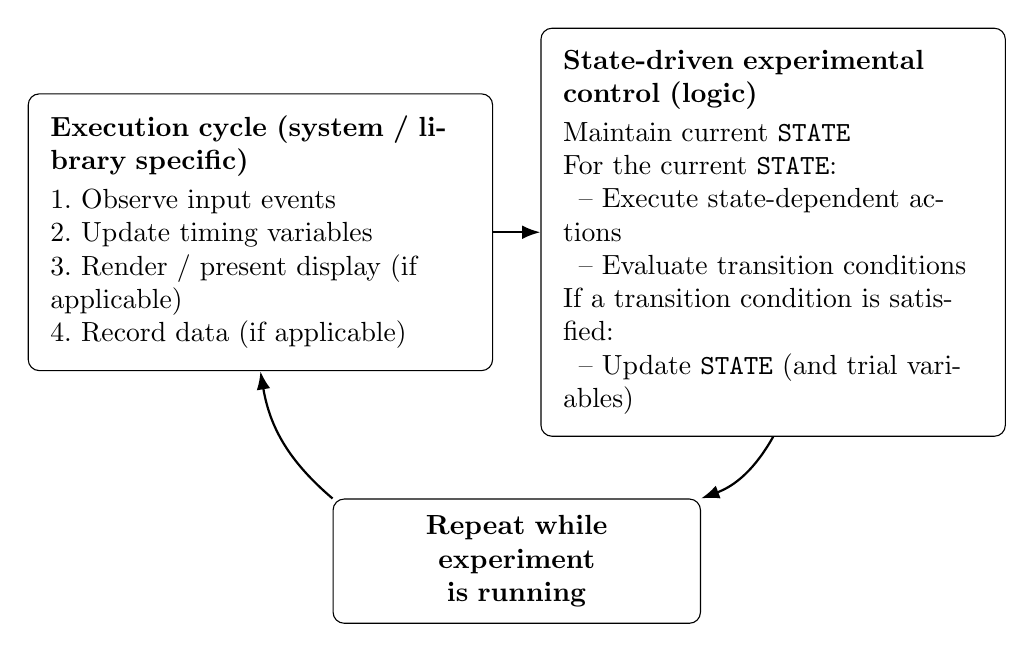
\begin{tikzpicture}[
  bigbox/.style={
    draw, rounded corners, align=left, inner sep=8pt,
    text width=0.44\linewidth
  },
  box/.style={
    draw, rounded corners, align=center, inner sep=6pt
  },
  arrow/.style={-Latex, thick}
]

\node[bigbox] (loop) {
\textbf{Execution cycle (system / library specific)}\\[2pt]
1.\ Observe input events\\
2.\ Update timing variables\\
3.\ Render / present display (if applicable)\\
4.\ Record data (if applicable)
};

\node[bigbox, right=6mm of loop] (sm) {
\textbf{State-driven experimental control (logic)}\\[2pt]
Maintain current \texttt{STATE}\\
For the current \texttt{STATE}:\\
\hspace*{2mm}-- Execute state-dependent actions\\
\hspace*{2mm}-- Evaluate transition conditions\\
If a transition condition is satisfied:\\
\hspace*{2mm}-- Update \texttt{STATE} (and trial variables)
};

\coordinate (mid) at ($(loop.south)!0.5!(sm.south)$);

\node[box, below=12mm of mid, text width=0.35\linewidth] (repeat) {
\textbf{Repeat while experiment\\ is running}
};

\draw[arrow] (loop.east) -- (sm.west);
\draw[arrow] (sm.south) to[bend left=20] (repeat.north east);
\draw[arrow] (repeat.north west) to[bend left=20] (loop.south);

\end{tikzpicture}
\caption{Separation between system-dependent execution operations
(e.g., event polling, timing, rendering, logging) and the
system-independent logic of state-driven experimental control.}
\label{fig:execution_cycle}
\end{figure}

The previous sections introduced behavioural experiments as
state-driven systems and described the general structure
through which experimental behaviour can be represented in
terms of states and transitions. The purpose of the present
section is to demonstrate how common behavioural paradigms
can be expressed within this framework by varying state
definitions and transition conditions. The examples that
follow illustrate the generality of the formulation rather
than serving as implementation guides.

Complete, runnable implementations accompanying this paper
are provided in a companion repository that serves as a
reference implementation of the state-driven framework
described here . The repository contains equivalent task
implementations across multiple programming environments,
illustrating how the same experimental structure can be
realized independently of specific presentation backends.
The repository can be found here: \url{\CompanionRepo}

\subsection{Reaction Time Task}

A simple reaction time task provides a minimal example of a
complete behavioural experiment expressed within the
state-driven framework. The task consists of a fixation
period followed by stimulus presentation, a response window,
feedback, and an inter-trial interval. These phases map
directly onto states, while transitions between states are
governed by elapsed time and participant input.

Within this formulation, reaction time arises naturally from
a transition between states. Stimulus onset corresponds to
entry into the stimulus state, and response latency
corresponds to the time elapsed before a transition from the
stimulus state to the feedback state occurs. Experimental
structure is therefore defined by the conditions governing
these transitions rather than by the sequential ordering of
commands.

\begin{tcolorbox}[title=Reaction Time Task Pseudocode]
\begin{Verbatim}[fontsize=\small]
Initialize STATE as FIXATION

Repeat while experiment is running:

    If STATE is FIXATION:
        present fixation stimulus

        If fixation duration has elapsed:
            present target stimulus
            start response timer
            STATE = STIMULUS

    Else if STATE is STIMULUS:
        present target stimulus

        If response detected:
            record response and reaction time
            STATE = FEEDBACK

        Else if response deadline exceeded:
            record missed response
            STATE = FEEDBACK

    Else if STATE is FEEDBACK:
        present feedback

        If feedback duration has elapsed:
            advance to next trial
            STATE = FIXATION
\end{Verbatim}
\end{tcolorbox}

This formulation makes explicit that stimulus presentation,
response collection, and feedback correspond to behaviours
associated with particular states rather than to independent
procedures executed once in sequence. Extensions to the
task—such as anticipatory responses, variable fixation
durations, or adaptive response deadlines—can be introduced
by modifying transition conditions or adding states without
changing the overall structure of experimental control.

\subsection{Category Learning Task}

Category learning tasks extend the same structure by
introducing transitions that depend on trial-specific
variables and response correctness. On each trial, a
stimulus belonging to one of several categories is
presented, the participant makes a response, and feedback is
provided contingent on the relationship between the response
and the stimulus category.

Within the state-driven formulation, the task is again
expressed as a set of states connected by transition
conditions. A minimal version of the task consists of
stimulus presentation, response collection, feedback, and
an inter-trial interval, with transitions determined by both
participant input and task variables associated with the
current trial.

\begin{tcolorbox}[title=Category Learning Task Pseudocode]
\begin{Verbatim}[fontsize=\small]
Initialize STATE as STIMULUS
Select stimulus for current trial

Repeat while experiment is running:

    If STATE is STIMULUS:
        present stimulus

        If response detected:
            determine correctness
            record response and accuracy
            STATE = FEEDBACK

    Else if STATE is FEEDBACK:
        present feedback based on correctness

        If feedback duration has elapsed:
            select next stimulus
            STATE = STIMULUS
\end{Verbatim}
\end{tcolorbox}

Here, learning emerges from the interaction between state
transitions and trial-dependent variables rather than from
changes to the underlying structure used to represent
experimental control. Modifying feedback rules or
introducing probabilistic reinforcement requires changes to
state definitions or transition logic while leaving the
overall framework intact.

\subsection{Reaching Task}

A reaching task provides an example in which transitions
between states depend on continuously evaluated input rather
than on discrete events or fixed time intervals. In a
typical reaching experiment, participants move a cursor from
a start location toward one of several possible targets.
Movement onset, target acquisition, and feedback correspond
to distinct phases of the task, while transitions between
these phases depend on spatial conditions evaluated
continuously during task performance.

Within the state-driven formulation, the task can again be
described as a set of states connected by transition
conditions. A minimal version includes a start state, a
movement state, a feedback state, and an inter-trial
interval, with transitions determined by spatial criteria.

\begin{tcolorbox}[title=Reaching Task Pseudocode]
\begin{Verbatim}[fontsize=\small]
Initialize STATE as START
Select target for current trial

Repeat while experiment is running:

    If STATE is START:
        present start position

        If cursor enters start region:
            record movement onset time
            STATE = MOVE

    Else if STATE is MOVE:
        present target

        If cursor enters target region:
            record movement time
            STATE = FEEDBACK

        Else if movement deadline exceeded:
            record failed trial
            STATE = FEEDBACK

    Else if STATE is FEEDBACK:
        present feedback

        If feedback duration has elapsed:
            select next target
            STATE = START
\end{Verbatim}
\end{tcolorbox}

In this example, transitions depend on continuously evaluated
spatial variables rather than discrete responses or fixed
durations. The framework accommodates this change by altering
transition conditions rather than the structure used to
describe experimental control.

Taken together, the reaction time, category learning, and
reaching examples illustrate that a wide range of behavioural
paradigms can be expressed within a common state-driven
framework. Differences between tasks arise from differences
in state definitions and transition logic, while the
structure used to represent experimental behaviour remains
consistent across paradigms.

\section{Discussion}

The present work proposes that behavioural experiments can
be usefully represented as state-driven systems in which
experimental behaviour is defined by task states and the
conditions governing transitions between them. The primary
contribution is not a new programming technique or software
framework, but an explicit formulation of a representation
for experimental control that is already compatible with a
wide range of existing implementations. Making this
structure explicit provides a common way of reasoning about
experimental design and task behaviour that applies across
programming languages, experiment-building tools, and
experimental paradigms.

\subsection{Implications for experimental design and implementation}

Viewing experiments in terms of states and transitions
clarifies the relationship between experimental design and
program behaviour. Sequential descriptions specify the
intended order of events, but as task requirements expand,
the conditions governing progression between phases may
become distributed across multiple parts of an
implementation. Representing experimental phases explicitly
as states localizes these conditions, allowing all possible
outcomes associated with a phase of the task to be inspected
and modified in a single place.

This representation is particularly useful in experiments
that involve branching logic, timing constraints, adaptive
behaviour, or multiple competing outcomes. Early responses,
response deadlines, or trial-dependent feedback can be
expressed directly as alternative transitions rather than as
procedural checks inserted at multiple points in a sequence.
As a result, extensions to existing paradigms can often be
implemented by modifying transition conditions or state
definitions without restructuring the overall task logic.

The framework also separates experimental logic from
implementation details. Rendering, input handling, and data
recording determine how experimental behaviour is realized
within specific hardware and software environments, but they
do not define the structure of experimental control itself.
The same experimental structure can therefore be realized
across different tools while preserving the logic governing
task behaviour.

\subsection{Relationship to sequential approaches}

The state-driven formulation should not be understood as an
alternative to sequential implementations, but as a way of
making explicit the structure of experimental control that
sequential descriptions often leave implicit. Sequential
code provides a concise and intuitive representation for
linear procedures, and for many paradigms this approach is
entirely appropriate.

The distinction emphasized here is therefore not between
correct and incorrect implementation styles, but between
implicit and explicit representations of task structure.
Sequential approaches encapsulate transition logic within
procedural steps or helper functions, whereas state-driven
formulations represent transitions directly at the level of
experimental structure. For simple linear tasks the
difference may be largely conceptual; as task complexity
increases, explicitly representing states and transition
conditions can simplify reasoning about task flow by
localizing the conditions that determine behavioural change.

\subsection{Timing considerations}

Discussions of experiment implementation often associate
particular programming styles with improved timing
precision. In practice, timing accuracy is determined
primarily by how display updates, input polling, and
hardware synchronization are handled by the underlying
system rather than by the control-flow abstraction used to
describe experimental logic
\citep{plant_could_2013, bridges_timing_2020}. Display
updates are typically synchronized to refresh cycles through
buffer swaps or frame flips that block execution until the
next refresh interval, and this mechanism operates
independently of whether experimental control is expressed
sequentially or through an explicit state-based structure.

Within the present framework, timing is therefore treated as
an empirical property of the running system rather than as a
consequence of program structure. State transitions occur
when measured conditions are satisfied, whether those
conditions involve elapsed time, participant input, or
continuously evaluated variables. This perspective
emphasizes validation and measurement of timing behaviour
rather than reliance on particular implementation patterns.

\subsection{Graphical and programming-based environments}

The distinction developed in this work is independent of the
choice between graphical experiment builders and
programming-based frameworks. Graphical tools have
substantially increased the accessibility of experiment
construction and provide efficient workflows for many
standard paradigms \citep{mathot_opensesame_2012,
peirce_psychopypsychophysics_2007}, while scripting
environments offer direct access to program structure and
behaviour. In practice, both approaches frequently coexist,
for example when graphical task descriptions are extended
through embedded code to implement more complex logic.

From the perspective developed here, these environments
differ primarily in how explicitly the structure of
experimental control is represented. Many graphical tools
internally rely on state-based mechanisms, but transitions
between task phases may be distributed across interface
elements or encapsulated within software abstractions.
Making the underlying state-driven structure explicit
provides a common conceptual framework for reasoning about
experimental behaviour across both graphical and
programming-based environments.

\subsection{Explicit representations and AI-assisted development}

Recent advances in AI-assisted programming have made it
possible to generate functional experimental code from
high-level descriptions. This development does not eliminate
the need for explicit representations of experimental
structure, but instead increases their importance. Systems
that generate code must still be guided by a clear
specification of task logic, including the phases of the
experiment and the conditions under which behaviour changes.

The state-driven formulation described here provides such a
specification by separating experimental logic from
implementation details. Whether an experiment is implemented
manually, constructed using graphical tools, or generated
through AI-assisted workflows, representing experimental
behaviour in terms of states and transitions makes task
structure explicit and reduces ambiguity in how experimental
design is translated into program behaviour. In this sense,
the framework functions not only as a programming approach
but as a descriptive scaffold that can guide both human and
automated implementation.

\subsection{Limitations and scope}

The framework presented here is conceptual rather than
prescriptive. Many experiments can be implemented
effectively using higher-level abstractions or graphical
experiment builders, and the goal is not to replace existing
tools or development practices. Instead, the framework is
intended as a way of reasoning about experimental control
that can inform design decisions and clarify the structure
of experimental behaviour.

The examples presented focus on interactive behavioural
experiments with clearly defined task phases. Other
experimental contexts, including asynchronous or distributed
experimental systems, may require extensions or alternative
representations. Future work may explore how state-driven
formulations interact with web-based experimental platforms
or parallel control systems in which multiple processes
operate concurrently.

\subsection{Conclusion}

Behavioural experiments are commonly described as sequences
of events, but their behaviour is determined by conditions
that govern transitions between phases of a task.
Representing experimental control explicitly in terms of
states and transitions provides a unified way of reasoning
about how experimental design relates to task behaviour. By
articulating this framework explicitly, the present work
offers a transferable perspective on experimental control
that generalizes across tools, programming environments, and
experimental paradigms.

\bibliographystyle{apalike}
\bibliography{citations}

\end{document}
